% Compilar con pdfLaTeX

\documentclass[12pt,a4paper]{article}

% ------------------------------------------------
% PAQUETES
% ------------------------------------------------
\usepackage[utf8]{inputenc}
\usepackage[T1]{fontenc}
\usepackage[spanish]{babel}
\usepackage{geometry}
\usepackage{array}
\usepackage{longtable}
\usepackage{booktabs}
\usepackage{tabularx}
\usepackage{enumitem}
\usepackage{setspace}
\usepackage{titlesec}
\usepackage{hyperref}
\usepackage[table]{xcolor}
\usepackage{graphicx}
\usepackage{float}

\geometry{
    left=2.5cm,
    right=2.5cm,
    top=2.5cm,
    bottom=2.5cm
}

\setstretch{1.15}
\setlength{\parindent}{0pt}
\setlength{\parskip}{6pt}

\hypersetup{
    colorlinks=true,
    linkcolor=black,
    urlcolor=blue,
    citecolor=black
}

\renewcommand{\arraystretch}{1.35}

% ------------------------------------------------
% ESTILO DE TABLAS
% ------------------------------------------------
\definecolor{azulTabla}{RGB}{31, 78, 121}
\definecolor{azulClaroTabla}{RGB}{232, 240, 248}
\definecolor{grisTabla}{RGB}{245, 247, 250}
\definecolor{lineaTabla}{RGB}{190, 200, 210}

\setlength{\tabcolsep}{5.5pt}
\setlength{\extrarowheight}{3pt}
\setlength{\LTpre}{8pt}
\setlength{\LTpost}{8pt}
\arrayrulecolor{lineaTabla}

% ------------------------------------------------
% DOCUMENTO
% ------------------------------------------------
\begin{document}

% ------------------------------------------------
% CARÁTULA
% ------------------------------------------------
\begin{titlepage}
    \centering

    % Encabezado institucional
    {\large\textbf{UNIVERSIDAD TÉCNICA ESTATAL DE QUEVEDO}}\\[0.3cm]

    {\normalsize Facultad de Ciencias de la Ingeniería}\\[0.15cm]
    {\normalsize Carrera de Ingeniería de Software}

    \vspace{1.5cm}

    % Separador superior
    {\color{azulTabla}\rule{0.85\textwidth}{1.5pt}}

    \vspace{1.2cm}

    % Identificación de la actividad
    {\large\textcolor{azulTabla}{\textbf{ACTIVIDAD ACADÉMICA}}}\\[0.5cm]

    {\Large\textbf{FORM-TL-01}}\\[0.8cm]

    % Título principal
    {\LARGE\bfseries
    Clasificación y análisis\\[0.2cm]
    de requisitos
    }

    \vspace{0.5cm}

    {\large Plataforma de gestión de citas médicas}

    \vspace{1.2cm}

    % Separador inferior
    {\color{azulTabla}\rule{0.85\textwidth}{1.5pt}}

    \vspace{0.8cm}

    % Información académica
    \begin{minipage}{0.78\textwidth}
        \renewcommand{\arraystretch}{1.8}
        \begin{tabular}{@{}>{\bfseries}p{3.5cm}p{8cm}@{}}
            Asignatura: & Ingeniería de Requerimientos \\

            Código: & ISR-401 \\

            Estudiante: & Joseph Orlando Saltos Tello \\

            Curso: & Cuarto semestre de Software A \\

            Docente: & Gleiston Cicerón Guerrero Ulloa, PhD \\

            Fecha de entrega: & 31/10/2026
        \end{tabular}
    \end{minipage}

    \vfill

    % Pie de página
    {\color{azulTabla}\rule{0.85\textwidth}{0.8pt}}\\[0.4cm]

    {\normalsize\textbf{QUEVEDO -- LOS RÍOS -- ECUADOR}}\\[0.15cm]
    {\normalsize 2026}

\end{titlepage}

% ------------------------------------------------
% INTRODUCCIÓN
% ------------------------------------------------
\section{Introducción}

El presente trabajo desarrolla el análisis de los enunciados
correspondientes a una plataforma de gestión de citas médicas
para el Policlínico Ribera del Quevedo.

El propósito es identificar y clasificar los requisitos
planteados para el sistema, considerando su tipo, naturaleza
y nivel de aplicación. Además, se revisan aquellos enunciados
relacionados con la calidad que presentan expresiones
generales o poco precisas, con el fin de reformularlos
mediante condiciones que permitan comprobar su cumplimiento.

Finalmente, se realiza una comparación con el documento
elaborado por otro estudiante, identificando las diferencias
en el enfoque y en los criterios utilizados para organizar
los requisitos.

% ------------------------------------------------
% CLASIFICACIÓN DE REQUISITOS
% ------------------------------------------------
\section{Clasificación de los requisitos}

En esta sección se presenta la clasificación de los veinte
enunciados del caso de estudio. Para cada uno se identifica
su tipo, naturaleza y nivel, junto con una justificación
breve de la decisión tomada.

\small

\begin{longtable}{@{}
    >{\raggedright\arraybackslash}p{0.65cm}
    >{\raggedright\arraybackslash}p{3.8cm}
    >{\raggedright\arraybackslash}p{1.55cm}
    >{\raggedright\arraybackslash}p{1.45cm}
    >{\raggedright\arraybackslash}p{1.25cm}
    >{\raggedright\arraybackslash}p{5.0cm}
@{}}
\caption{Clasificación de los enunciados del caso de estudio}\\
\toprule
\rowcolor{azulTabla}
\color{white}\textbf{ID} &
\color{white}\textbf{Enunciado} &
\color{white}\textbf{Tipo} &
\color{white}\textbf{Naturaleza} &
\color{white}\textbf{Nivel} &
\color{white}\textbf{Justificación} \\
\midrule
\endfirsthead

\multicolumn{6}{c}{\small\textit{Continuación de la tabla anterior}}\\
\toprule
\rowcolor{azulTabla}
\color{white}\textbf{ID} &
\color{white}\textbf{Enunciado} &
\color{white}\textbf{Tipo} &
\color{white}\textbf{Naturaleza} &
\color{white}\textbf{Nivel} &
\color{white}\textbf{Justificación} \\
\midrule
\endhead

\midrule
\multicolumn{6}{r}{\small\textit{Continúa en la siguiente página}}\\
\endfoot

\bottomrule
\endlastfoot

\rowcolors{2}{azulClaroTabla}{white}

E01 &
El paciente reserva una cita seleccionando especialidad,
médico, fecha y hora entre los espacios disponibles. &
Funcional &
Producto &
Sistema &
Describe una función principal que permite al paciente
gestionar una cita médica mediante la plataforma. \\
\hline

E02 &
La plataforma envía al paciente un recordatorio por SMS
24 horas antes de la cita. &
Funcional &
Producto &
Software &
Establece una acción automática que debe ejecutar el
software para notificar al paciente. \\
\hline

E03 &
La aplicación debe ser rápida. &
Calidad
(eficiencia de desempeño) &
Producto &
Software &
Establece una expectativa sobre el rendimiento de la
aplicación, pero no especifica un tiempo máximo de respuesta. \\
\hline

E04 &
El recepcionista registra la llegada del paciente en el
mostrador. &
Funcional &
Producto &
Sistema &
Define una operación que debe realizarse durante el
proceso de atención al paciente. \\
\hline

E05 &
La plataforma debe desarrollarse con Java 21 y PostgreSQL,
tecnologías conocidas por el equipo de TI. &
Restricción &
Producto &
Software &
Limita las tecnologías que pueden utilizarse para
desarrollar e implementar el software. \\
\hline

E06 &
El médico consulta la lista de pacientes del día y marca
cada consulta como atendida. &
Funcional &
Producto &
Software &
Describe operaciones que el sistema debe ofrecer al
personal médico durante la jornada de trabajo. \\
\hline

E07 &
Los datos de salud de los pacientes deben estar seguros. &
Calidad
(seguridad) &
Producto &
Software &
Expresa una condición de seguridad, pero no establece
medidas ni criterios verificables para comprobarla. \\
\hline

E08 &
La aplicación móvil debe funcionar en Android 10 o superior. &
Restricción &
Producto &
Software &
Establece las versiones del sistema operativo compatibles
con la aplicación móvil. \\
\hline

E09 &
Las citas canceladas con menos de cuatro horas de
anticipación se registran como inasistencias. &
Funcional &
Producto &
Sistema &
Define una regla de negocio que determina cómo debe
registrarse una cancelación tardía. \\
\hline

E10 &
La aplicación debe ser fácil de utilizar para pacientes
de edad avanzada. &
Calidad
(usabilidad) &
Producto &
Software &
Se refiere a la facilidad de uso de la aplicación, pero
no define cómo se medirá dicha facilidad. \\
\hline

E11 &
El proyecto debe entregarse en un plazo máximo de seis meses. &
Restricción &
Proceso &
Sistema &
Establece un límite de tiempo para la ejecución y entrega
del proyecto de desarrollo. \\
\hline

E12 &
La sesión del usuario se cierra automáticamente después
de diez minutos de inactividad. &
Funcional &
Producto &
Software &
Define el comportamiento automático del sistema cuando
un usuario permanece inactivo durante un periodo determinado. \\
\hline

E13 &
El kiosco de la sala de espera lee el número de identificación
ingresado en la pantalla táctil e imprime un ticket con
el número de turno. &
Funcional &
Producto &
Sistema &
Describe una operación que involucra componentes de
software y dispositivos físicos del sistema. \\
\hline

E14 &
La aplicación debe estar siempre disponible. &
Calidad
(fiabilidad) &
Producto &
Sistema &
Expresa una expectativa de disponibilidad, pero no
establece un porcentaje ni un periodo de medición. \\
\hline

E15 &
El director médico puede generar un informe mensual de
inasistencias por especialidad. &
Funcional &
Producto &
Software &
Establece una función de generación de informes para
consultar información sobre las inasistencias. \\
\hline

E16 &
Cada incremento debe validarse con el director médico
al finalizar cada iteración de dos semanas. &
Restricción &
Proceso &
Sistema &
Establece una condición que debe cumplirse durante
el proceso de desarrollo y validación del proyecto. \\
\hline

E17 &
El tratamiento de datos personales debe cumplir con la
Ley Orgánica de Protección de Datos Personales de Ecuador. &
Restricción &
Producto &
Sistema &
Establece una obligación legal que debe respetar la
solución durante el tratamiento de datos personales. \\
\hline

E18 &
La plataforma debe integrarse sin inconvenientes con el
sistema de facturación actual, que dispone de servicios
web documentados y no será reemplazado. &
Calidad
(compatibilidad) &
Producto &
Software &
Se refiere a la interoperabilidad con un sistema externo,
pero la expresión ``sin inconvenientes'' no establece
condiciones verificables. \\
\hline

E19 &
Si falla el servidor principal, el servicio debe recuperarse
en menos de 30 minutos sin perder las citas confirmadas. &
Calidad
(fiabilidad) &
Producto &
Sistema &
Establece condiciones de recuperación ante fallos y
conservación de la información de las citas. \\
\hline

E20 &
Cada cambio del código fuente debe ser revisado por otro
integrante del equipo antes de incorporarse a la rama principal. &
Restricción &
Proceso &
Software &
Establece una condición obligatoria para el control de
cambios durante el desarrollo del software. \\
\hline
\end{longtable}

\normalsize

% ------------------------------------------------
% REQUISITOS DE CALIDAD VAGOS
% ------------------------------------------------
\section{Identificación y reformulación de requisitos de calidad}

Se identificaron cinco enunciados relacionados con la
calidad que presentan expresiones generales o ambiguas.
Estas expresiones dificultan comprobar si el requisito
se cumple, debido a que no establecen valores o condiciones
específicas de evaluación.

Por esta razón, se proponen reformulaciones que incorporan
métricas, unidades y umbrales para facilitar su verificación.

\subsection{Requisito E03: Rendimiento}

\textbf{Enunciado original:}

La aplicación debe ser rápida.

\textbf{Problema identificado:}

El término ``rápida'' es subjetivo, porque no indica cuánto
tiempo debe tardar la aplicación en responder a las acciones
realizadas por los usuarios.

\textbf{Requisito reformulado:}

La plataforma deberá responder a las operaciones principales
de consulta y registro en un tiempo máximo de 2 segundos
en al menos el 95\% de las solicitudes, bajo una carga de
300 usuarios simultáneos.

\textbf{Métrica:} Tiempo de respuesta.

\textbf{Unidad:} Segundos.

\textbf{Umbral:} Máximo 2 segundos en al menos el 95\%
de las solicitudes.

\subsection{Requisito E07: Seguridad}

\textbf{Enunciado original:}

Los datos de salud de los pacientes deben estar seguros.

\textbf{Problema identificado:}

El enunciado no especifica qué mecanismos deben aplicarse
para proteger los datos ni cómo se comprobará que el acceso
a esta información se encuentre controlado.

\textbf{Requisito reformulado:}

El sistema deberá exigir autenticación y verificar los
permisos del usuario antes de permitir el acceso a los
datos de salud de los pacientes. El 100\% de las pruebas
de acceso a información protegida deberá impedir el ingreso
de usuarios no autorizados.

\textbf{Métrica:} Porcentaje de pruebas de acceso no autorizado
bloqueadas correctamente.

\textbf{Unidad:} Porcentaje.

\textbf{Umbral:} 100\% de las pruebas realizadas.

\subsection{Requisito E10: Usabilidad}

\textbf{Enunciado original:}

La aplicación debe ser fácil de utilizar para pacientes
de edad avanzada.

\textbf{Problema identificado:}

La expresión ``fácil de utilizar'' no define qué nivel
de facilidad debe alcanzar la aplicación ni cómo se
evaluará la experiencia de los pacientes mayores.

\textbf{Requisito reformulado:}

Al menos el 90\% de los pacientes mayores que participen
en las pruebas de usabilidad deberá completar el proceso
de reserva de una cita médica en un tiempo máximo de
3 minutos, sin recibir ayuda de otra persona.

\textbf{Métrica:} Porcentaje de participantes que completan
la reserva correctamente.

\textbf{Unidad:} Porcentaje y minutos.

\textbf{Umbral:} Al menos 90\% de participantes y máximo
3 minutos por reserva.

\subsection{Requisito E14: Disponibilidad}

\textbf{Enunciado original:}

La aplicación debe estar siempre disponible.

\textbf{Problema identificado:}

La palabra ``siempre'' representa una condición difícil
de medir, porque no establece un porcentaje de disponibilidad
ni un periodo concreto para realizar la evaluación.

\textbf{Requisito reformulado:}

La plataforma deberá mantener una disponibilidad mensual
mínima del 99,5\% durante el horario de atención del
policlínico, comprendido entre las 07:00 y las 19:00,
de lunes a sábado.

\textbf{Métrica:} Porcentaje de disponibilidad.

\textbf{Unidad:} Porcentaje mensual.

\textbf{Umbral:} Disponibilidad mínima del 99,5\%.

\subsection{Requisito E18: Compatibilidad}

\textbf{Enunciado original:}

La plataforma debe integrarse sin inconvenientes con el
sistema de facturación actual.

\textbf{Problema identificado:}

La expresión ``sin inconvenientes'' no determina qué
condiciones debe cumplir la integración ni cómo se
comprobará que la comunicación entre ambos sistemas
funcione correctamente.

\textbf{Requisito reformulado:}

La plataforma deberá intercambiar correctamente la
información definida para la integración con el sistema
de facturación actual. El 100\% de los casos de prueba
de integración establecidos deberá completarse
correctamente, sin pérdida ni alteración de los datos
transmitidos.

\textbf{Métrica:} Porcentaje de casos de prueba de integración
aprobados.

\textbf{Unidad:} Porcentaje.

\textbf{Umbral:} 100\% de los casos de prueba aprobados,
sin pérdida ni alteración de datos.

% ------------------------------------------------
% COMPARACIÓN CON OTRO ESTUDIANTE
% ------------------------------------------------
\section{Análisis comparativo con otro compañero}

Se realizó una revisión del documento elaborado por el compañero MORAN PILAGUANO FRIXON FERNANDO. La comparación permitió identificar
diferencias en el contenido y en la forma de organizar
los requisitos.

Aunque ambos trabajos presentan veinte enunciados, estos
no corresponden a los mismos requisitos. El documento
revisado aborda principalmente aspectos relacionados con
la gestión de usuarios, bases de datos, seguridad,
documentación, pruebas y control del desarrollo. En cambio,
el presente trabajo se basa en los enunciados establecidos
para la plataforma de gestión de citas médicas del
Policlínico Ribera del Quevedo.

\subsection{Diferencias identificadas}

\begin{longtable}{@{}
    >{\raggedright\arraybackslash}p{2.8cm}
    >{\raggedright\arraybackslash}p{5.3cm}
    >{\raggedright\arraybackslash}p{5.3cm}
@{}}
\toprule
\rowcolor{azulTabla}
\color{white}\textbf{Aspecto} &
\color{white}\textbf{Presente trabajo} &
\color{white}\textbf{Documento del otro estudiante} \\
\midrule
\endfirsthead

\multicolumn{3}{c}{\small\textit{Continuación de la tabla anterior}}\\
\toprule
\rowcolor{azulTabla}
\color{white}\textbf{Aspecto} &
\color{white}\textbf{Presente trabajo} &
\color{white}\textbf{Documento del otro estudiante} \\
\midrule
\endhead

\midrule
\multicolumn{3}{r}{\small\textit{Continúa en la siguiente página}}\\
\endfoot

\bottomrule
\endlastfoot

\rowcolors{2}{azulClaroTabla}{white}

Contenido &
Se centra en la reserva, atención, cancelación y
administración de citas médicas, además de las
condiciones de calidad y restricciones del caso. &
Incluye enunciados relacionados con usuarios, bases
de datos, auditoría, pruebas, documentación y
mantenimiento del software. \\
\hline

Criterios de clasificación &
Se identifica el tipo de requisito, su naturaleza
y su nivel de aplicación. &
Se utilizan categorías de requisitos y una
clasificación de prioridad mediante MoSCoW. \\
\hline

Enfoque &
Se analiza una solución destinada a gestionar los
servicios de atención médica del policlínico. &
Se abordan diferentes aspectos técnicos y de
organización para el desarrollo de un sistema. \\
\hline

Organización &
Cada enunciado se acompaña de una justificación
que explica su clasificación. &
Los enunciados se organizan mediante su descripción,
categoría, prioridad y justificación. \\
\hline
\end{longtable}

\subsection{Discrepancias y resolución}

No fue posible establecer discrepancias individuales
entre los requisitos E01--E20 de ambos documentos, debido
a que los enunciados no son equivalentes ni describen
las mismas funcionalidades o condiciones.

La diferencia principal se encuentra en el contenido
analizado y en los criterios de clasificación empleados.
Por lo tanto, se mantuvo como base del presente trabajo
el conjunto de enunciados proporcionado para el caso
de la plataforma de gestión de citas médicas.

La comparación permitió reconocer que ambos documentos
organizan y justifican requisitos, pero responden a
contextos y criterios de análisis diferentes. No se
modificaron los enunciados del caso de estudio para
hacerlos coincidir con los del otro documento.

% ------------------------------------------------
% DECLARACIÓN DE USO DE IA
% ------------------------------------------------
\section{Declaración de uso responsable de IA}

Para la elaboración de este trabajo se utilizó una
herramienta de inteligencia artificial como apoyo en
actividades específicas de organización y revisión
del documento.

Su utilización se limitó a las siguientes actividades:

\begin{itemize}
    \item Apoyo en el diseño y organización del documento
    mediante LaTeX.
    \item Asistencia para mejorar la redacción de algunos
    apartados, manteniendo el significado de los
    enunciados originales.
    \item Revisión de errores ortográficos, gramaticales
    y de puntuación.
\end{itemize}

\subsection*{Ejemplos de prompts utilizados}

\begin{enumerate}
    \item ``Ayúdame a mejorar el diseño visual de mi documento
en LaTeX para que tenga una presentación académica
ordenada y profesional. Recomiéndame una tipografía
adecuada, el tamaño de letra para los títulos,
subtítulos y enunciados, la distribución de los
elementos en las páginas, los márgenes, el espaciado
entre párrafos y líneas, y el formato de las tablas.
También ayúdame a definir la alineación de los textos,
la jerarquía visual de los encabezados y la presentación
de la portada, buscando que todo el documento mantenga
un estilo uniforme y sea fácil de leer.Ayúdame a organizar el documento en LaTeX
    para presentar la clasificación y el análisis de
    los requisitos de manera clara y ordenada.''
\begin{figure}[H]
    \centering
    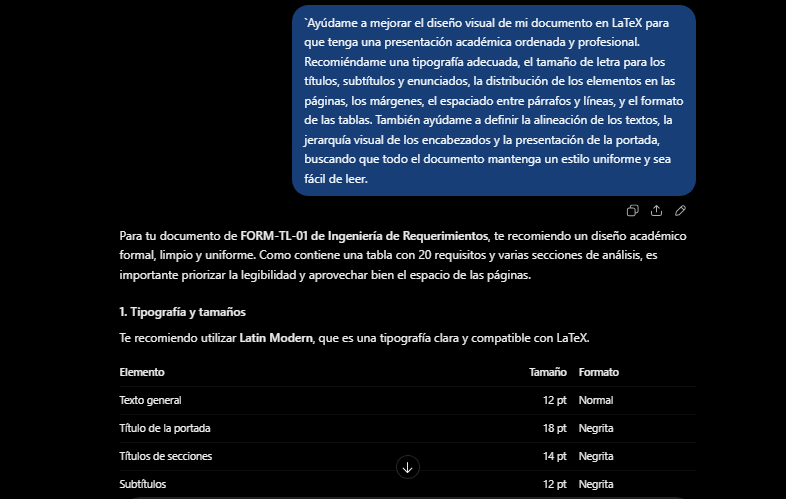
\includegraphics[width=0.9\textwidth]{1.png}
    \caption{Prompt acerca del diseño y estilo del documento.}
    \label{fig:clasificacion}
\end{figure}
\clearpage
    \item ``Revisa la redacción de los apartados de mi
    trabajo sobre la clasificación y análisis de
    requisitos de una plataforma de gestión de citas
    médicas. Ayúdame a mejorar la claridad, coherencia
    y formalidad de los párrafos, utilizando un lenguaje
    académico sencillo y evitando repeticiones. Conserva
    el significado de los enunciados originales y no
    agregues información que no esté relacionada con
    el caso de estudio.''
\begin{figure}[H]
    \centering
    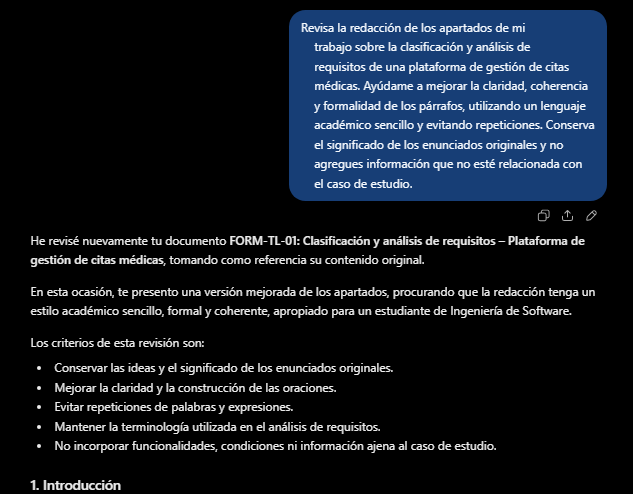
\includegraphics[width=0.9\textwidth]{2.png}
    \caption{Revision de la sección de clasificación y análisis de requisitos.}
    \label{fig:clasificacion}
\end{figure}
\clearpage
    \item ``Realiza una revisión ortográfica y gramatical
    del contenido de mi documento académico. Identifica
    errores en la escritura, acentuación, concordancia,
    puntuación y construcción de las oraciones. Indica
    las correcciones necesarias para mejorar la
    presentación del trabajo, procurando conservar
    las ideas originales y el sentido de cada apartado.''
    \begin{figure}[H]
    \centering
    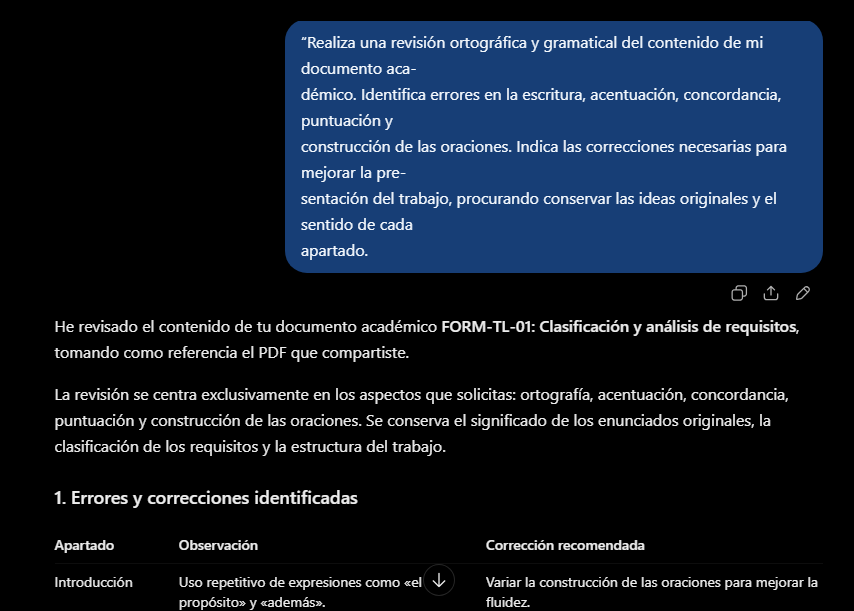
\includegraphics[width=0.9\textwidth]{3.png}
    \caption{Revisión ortográfica y gramatical del documento.}
    \label{fig:clasificacion}
\end{figure}
\end{enumerate}



% ------------------------------------------------
% REFERENCIAS
% ------------------------------------------------
\section{Referencias}

\begin{thebibliography}{9}

\bibitem{iso25010}
International Organization for Standardization,
\textit{ISO/IEC 25010:2011 Systems and software engineering
-- Systems and software Quality Requirements and Evaluation
(SQuaRE) -- System and software quality models}.
Geneva, Switzerland: ISO, 2011.

\bibitem{lopdp}
Asamblea Nacional del Ecuador,
\textit{Ley Orgánica de Protección de Datos Personales},
Registro Oficial Suplemento No. 459, 26 de mayo de 2021.

\end{thebibliography}

\end{document}